\documentclass[acmtoms,acmnow]{acmtrans2m}
\usepackage{graphicx}
\newcommand{\bsinglespace}{\renewcommand{\baselinestretch}{1.2}\small\normalsize}
\newcommand{\esinglespace}{}
\markboth{Michael A. Heroux et al.}{An Overview of Trilinos}

\title{An Overview of the Trilinos Project}

\author{MICHAEL A. HEROUX \\ 
ROSCOE A. BARTLETT \\
VICKI E. HOWLE \\
ROBERT J. HOEKSTRA \\
JONATHAN J. HU \\
TAMARA G. KOLDA \\
RICHARD B. LEHOUCQ \\
KEVIN R. LONG \\
ROGER P. PAWLOWSKI \\
ERIC T. PHIPPS \\
ANDREW G. SALINGER \\
HEIDI K. THORNQUIST \\
RAY S. TUMINARO \\
JAMES M. WILLENBRING \\
ALAN WILLIAMS \\
Sandia National Laboratories \\
and \\
KENDALL S. STANLEY \\
Oberlin College}


\begin{abstract}
The Trilinos Project is an effort to facilitate the design, development, 
integration and ongoing support of mathematical software libraries within an 
object-oriented framework for the solution of large-scale, complex multi-physics 
engineering and scientific problems.  Trilinos addresses two fundamental issues 
of developing software for these problems: (i) Providing a streamlined process 
and set of tools for development of new algorithmic implementations and (ii) 
promoting interoperability of independently developed software.  

Trilinos uses a two-level software structure designed around
collections of
{\it packages}.  A Trilinos package is an integral unit usually
developed by a small team of experts in a particular algorithms area
such as algebraic preconditioners, nonlinear solvers, etc.  
Packages exist underneath
the Trilinos top level, which provides a common look-and-feel,
including configuration, documentation, licensing, and bug-tracking.

Here we present the overall Trilinos design, describing our use of 
abstract interfaces and default concrete implementations.  We discuss the 
services that Trilinos provides to a prospective package and how these services 
are used by various packages. We also illustrate how packages can be
combined to rapidly develop new algorithms.  Finally, we discuss how
Trilinos facilitates high-quality software engineering practices that
are increasingly required from simulation software.
\end{abstract}

\begin{document}

\category{G.1.3}{Numerical Analysis}{Numerical Linear Algebra}
\category{G.4}{Mathematics of Computing}{Mathematical Software}
\category{D.2.13}{Software Engineering}{Reusable Software}

\terms{Algorithms, Design, Performance, Reliability}

\keywords{Software framework, Interfaces, Software Quality Engineering}


\begin{bottomstuff}
Sandia is a multiprogram laboratory operated by Sandia Corporation, a
Lockheed-Martin Company, for the United States Department of Energy
under Contract DE-AC04-94AL85000.

\end{bottomstuff}

\maketitle


\section{Introduction}

Research efforts in advanced solution algorithms and parallel solver
libraries have historically had a large impact on engineering and
scientific computing.  Algorithmic advances increase the range
of tractable problems and reduce the cost of solving existing
problems.  Well-designed solver libraries provide a mechanism for
leveraging solver development across a broad set of applications and
minimize the cost of solver integration.  Emphasis is
required in both new algorithms and new software in order
to maximum the impact of our efforts.

Sandia has developed scalable solver algorithms and software for many years.  
Often this development has been done within the context of 
a specific application code, providing a good robust solver that 
meets the particular needs of that application.  Even Aztec~\cite{Aztec2.1}, one of 
the most important general-purpose solvers developed at Sandia, was 
developed specifically for MPSalsa~\cite{MPSalsa-User-Guide,MPSalsa-Theory} 
and only later extracted for use with other applications.  Unfortunately, 
even though application-focused solvers tend to be very robust and can 
often be made into very effective general-purpose solvers, the 
opportunity to re-use the basic set of tools developed for one solver 
in the development of another solver becomes very difficult.

The Trilinos Project grew out of this group of established numerical algorithms
efforts at Sandia, motivated by  a recognition that a modest degree of 
coordination across these efforts could have a large positive impact on 
the quality and usability of the software we produce and therefore enhance the
research, development and integration of new solver algorithms into
applications.  With the advent of Trilinos, the degree of effort required 
to develop new parallel solvers has been 
substantially reduced, because our common infrastructure provides an good 
starting point for new development.  Furthermore, many applications 
are standardizing on the 
Trilinos matrix and vector classes.  As a result, these applications
have access to all Trilinos capabilities without  
interface modifications. 

Trilinos has a two-level design where the fundamental building block
is a {\it package}.  Although package is a common term, we define it
rigorously within Trilinos.  Specifically, each package is a numerical
library (or collection of libraries) that is:
\begin{itemize}
\item Focused on important, state-of-the-art algorithms in its problem
regime.  For example: algebraic preconditioners, nonlinear solvers, 
scalable data models, etc.
\item Developed by a small team of domain experts.
\item Self-contained, with minimal dependencies on other packages.
\item Configurable, buildable, tested and documented on its own.
\end{itemize}
These packages can be distributed within Trilinos or separately. 
The Trilinos framework provides a common look-and-feel that 
includes configuration, documentation, licensing, and bug 
tracking.  There are also guidelines and tools for adding new packages 
to Trilinos. 

The Trilinos project encompasses a variety of efforts that are to some
extent self-contained but at the same time inter-related.  The
Trilinos design allows individual packages to grow and mature
autonomously to the extent the algorithms and package developers
dictate.  This document provides an overview of the project,
focusing on the project philosophy and description, and
providing the reader with a summary of the project in its current
state. 
Section~\ref{Sect:RelatedWork} discusses work that is related to Trilinos. 
Integration of a package into Trilinos, and what Trilinos can provide
to a package, will be discussed in Section~\ref{sect:TrilinosServices}.
Section~\ref{sect:Software} discusses the current collection of Trilinos
packages.  Section~\ref{sect:Interoperability} presents some code
fragments that illustrate the interoperability of Trilinos packages.
This section also discusses the Meros package in greater detail
because it illustrates how multiple Trilinos packages can be combined 
to quickly provide production implementations of state-of-the-art 
algorithms.  Finally, Section~\ref{sect:SQA} discusses the role of 
Trilinos to improve software quality and reduce the cost of software 
quality assurance processes, an increasingly important aspect
of computer modeling and simulation for science and engineering.  

\section{Related Work}
\label{Sect:RelatedWork}
General-purpose solver libraries have been used successfully across 
a broad set of applications and computer systems.  EISPACK~\cite{eispack}, 
LINPACK~\cite{linpack} and LAPACK~\cite{lapack} are just a few of
the many libraries that have made a tremendous impact, providing robust 
portable solvers to a broad set of applications.  More recently, libraries 
such as PETSc~\cite{petsc-home-page,petsc-manual,petsc-efficient}, 
ScaLAPACK~\cite{scalapack}, PLAPACK~\cite{plapack} 
and Aztec~\cite{Aztec2.1} have enabled development of parallel
applications by giving users access to parallel distributed 
memory solvers that are easy-to-use and robust.

The purpose of the Trilinos project is to foster development
of new solver libraries by minimizing the costs of new development,
while still leveraging the investment in
established libraries such as those just mentioned.  These two goals
are accomplished by active research and development of new libraries
and by use of the Trilinos package architecture.  Although
Trilinos is unique in design, a number of other projects have some 
similarities.  In particular, PETSc, the Common Component Architecture
(CCA)~\cite{CCA-home-page}, the Matrix
Template Library (MTL)~\cite{MTL-home-page} and POOMA~\cite{POOMA}
share attributes with Trilinos.

\subsection{Trilinos and PETSc}
Trilinos is similar to PETSc in that both provide libraries for
constructing and using sparse and dense distributed matrices and
vectors.  Also, both projects provide solver libraries for linear, nonlinear,
time-dependent and eigenvalue problems.  Trilinos differs from PETSc
in that Trilinos is written primarily in C++, has an explicit
modular architecture and each package is interoperable with other
packages but not interdependent.  Most Trilinos packages are
data-neutral in design and in fact could easily use PETSc libraries to
provide a variety of capabilities via straight-forward implementation
of documented abstract interfaces, without modifying PETSc or Trilinos source code.  

\subsection{Trilinos and the Common Component Architecture}
The Trilinos package architecture, which is the primary difference between
Trilinos and PETSc,
is the primary similarity between Trilinos and the CCA.  Like the CCA,
the Trilinos
package architecture supports interoperability of independent
pieces of software.  However, the CCA uses an advanced runtime
environment to manage the coupling of components, whereas Trilinos
uses configure-enabled conditional compilation and the polymorphism
that is inherent in the C++ language.  Both
approaches are essential and very compatible.  In fact, the modularity
and independence of Trilinos
packages make them easy to wrap as CCA components.

\subsection{Trilinos and MTL}
The Trilinos packages Epetra and Tpetra are similar to MTL.  All three
are written in C++ and provide numerical linear algebra objects
that can be used to implement numerical algorithms.  MTL
makes more aggressive use of template facilities in C++ and allows
more elegant and flexible implementations.  However, portability of
MTL is a major issue since a number of C++ compilers do not 
support some of
the features used by MTL.  Another difference is that MTL provides its
own functionality that is similar to the BLAS, whereas Epetra and
Tpetra rely on BLAS libraries for performance.  A final
major difference is that MTL executes on serial machines only.  
Epetra and Tpetra support distributed
memory objects and provide parallel data repartitioning
capabilities~\cite{Repartitioning}.

\subsection{Trilinos and POOMA}

Trilinos and POOMA are similar in that they both provide serial and parallel
distributed memory linear algebra objects, along with automatic support of
interprocessor communication.   POOMA differs from Trilinos in its
focus on arrays and overloaded operator syntax, which make
grid-based calculations and explicit methods easy to implement.  In
fact, much of POOMA terminology uses grid concepts.  POOMA also focuses
only on basic linear algebra computations.  No implicit solvers are
provided, although grid-based implicit solvers can be easily built
using POOMA objects.
Trilinos packages such as Epetra and Tpetra can be used for grid-based
computations, but their primary focus is on
irregular, unstructured computations.  Other Trilinos packages access
linear algebra services via abstract vector and operator interfaces.
Therefore, POOMA object could be used via these interfaces. 

\subsection{Trilinos and Other Solver Libraries}
Trilinos provides significant new solver capabilities as 
self-contained Trilinos packages.  It also provides an explicit,
documented, modular architecture that 
facilitates interoperability.  This allows Trilinos to easily use
other solver libraries and to also provide, via any individual Trilinos
package, solver capabilities to other libraries. External solver
libraries are made Trilinos-compatible, not by integrating them into
Trilinos, but by augmenting the capabilities of the external library.
This difference in design philosophy is subtle but important,
especially for scalable growth in package count.  Using this approach,
Trilinos will never become a large monolithic piece of software,
something that is very important as the volume of solver software
continues to grow.

\section{Trilinos Package Architecture and Services}
\label{sect:TrilinosServices}

In our experience mathematical libraries tend to be written by small
teams of domain experts.  For example, approximately 25 staff
members (not including students) contribute to Trilinos development 
across approximately 25
different packages, but most individual Trilinos packages
are developed by one to three staff members, and no single package 
has more than five
developers.   Some staff members contribute to more than one package,
but very few contribute to more than three packages.  Another
observation is that mathematical libraries tend to be written
by experienced numerical software
developers who do not have much, if any, experience with formal
software tools and processes.  Both of these observations have
motivated the Trilinos design and implementation.  The Trilinos
package architecture naturally supports small inter-related team
development efforts. Trilinos services, provided on a
package-by-package basis, directly address the second observation.

\subsection{Modularity via Packages}
Each Trilinos package is fully self-sufficient and self-contained,
unless there are explicit dependencies designed into a package.
Package source code and revision history is contained within a single directory
structure.  Mail lists, software faults, documentation, websites and
interoperability are all organized via packages.  

Package
interoperability is accomplished via configure-time enabling of
package-to-package coupling.  For example, IFPACK has many parameters
to control how preconditioners are constructed and used, e.~.g~.,
level of fill in an incomplete factorization.  Teuchos provides a
parameter list class that can be used to specify parameter values.
If the argument {\tt
--enable-teuchos} is specified when IFPACK is configured, Teuchos
ParameterList support will be compiled in IFPACK, otherwise this code
will not be enabled and only IFPACK's internal parameter setting
method is available.  Configure-time enabling of package
interoperability is commonly used for any optional package coupling
that makes sense.  In this way packages retain autonomy but can easily
be combined with any other package that makes sense algorithmically. 
 
\subsection{Package Services Provided by Trilinos}
Trilinos provides a variety of services to package
developers.  When a new package is introduced into Trilinos, each of
these services is established, immediately providing the new package
with necessary tools to address important software quality engineering
practices (see Section~\ref{sect:SQA} for details).  All tools are 
accessible from the main Trilinos website~\cite{Trilinos-home-page}.
Specifically the services we establish are: 

\begin{itemize}
\item {\bf Source code repository:}
Trilinos source code is
maintained in a CVS~\cite{CVS} repository that is accessible via a
secure connection from anywhere on the internet.  For most new
packages, use of a supported CVS repository is the most important
service Trilinos provides, since development is typically in the early
stages and there are few if any users.

\item {\bf Mail lists:}
Trilinos uses the Mailman~\cite{Mailman} list manager to provide
communication support for each package.  Package lists start with the
package name followed by the list function, e.~g.~, AztecOO-Announce.
The
following mail lists are established for each package:
\begin{itemize}
\item Package-Announce: All news related to this package is sent to
this list, such as release announcements, etc.
\item Package-Developers: Package developer discussions occur on this list,
including design and policy discussions.  Key development decisions are posted
here for archival purposes.
\item Package-Users: List for package users. General discussions about
use of the package are conducted here, typically monitored by the
package development team.
\item Package-Checkins: All log messages that are submitted with
source code changes to the CVS repository are sent to this list.
Anyone wishing to see the moment-to-moment activity in package
development can subscribe to this list.
\item Package-Regression: All output from the regression test suite
for the package is sent to this list.
\end{itemize}

\item {\bf Issue tracking:}
Bugzilla~\cite{Bugzilla} is a web-based issue tracking
application that supports submission and tracking of software issues,
including enhancements and faults.  Each package has its own Bugzilla
product.

\item {\bf Fault identification:}
Bonsai~\cite{Bonsai} is a web-based application that supports a
variety of CVS repository browsing capabilities, and links changes in the
repository to Bugzilla issues. Bonsai is most useful as a way to
quickly identify changes in source code that have cause a software
fault.

\item {\bf Configuration management:}
Autoconf~\cite{Autoconf},  Automake~\cite{Automake} and
Libtool~\cite{Libtool} provide a robust, full-featured set of tools for
building software across a broad set of platforms (see also the ``Goat
Book''~\cite{GoatBook}).  Although these
tools are not official standards, they are widely used.  All existing
Trilinos packages use Autoconf and Automake.  Libtool support will be
added in future releases. 

Trilinos provides a library of M4~\cite{M4} macros that can be used by any other
package that wants to use Autoconf and Automake for configuring and
building libraries.  These macros perform common configuration tasks such as
locating a valid LAPACK~\cite{lapack} library, checking for a
user-defined MPI~\cite{MPI} C compiler or determining inter-language linking
rules.  This library of macros minimizes the amount of redundant
 effort in using Autotools, and make it easier to apply a general change to
the configure process for all packages.

\item {\bf Automated Regression testing:} Trilinos provides a variety
of  regression testing capabilities.
Integrating new tests into Trilinos is accomplished by creating
specially named directories in the CVS repository and creating scripts
that run package tests.  For example, an executable script committed
to the repository in the directory 
Trilinos/packages/epetra/test/scripts/daily/serial can be executed manually and
will also run daily on any platform that has the Epetra serial test harness
installed, as part of the automated regression test harness.  On a nightly 
basis, the test harness builds the most recent versions of Trilinos libraries 
and runs any tests that are present in one of these special directories.  
\end{itemize}

\subsection{The new\_package Package} 

In order to reduce the start up time for a new Trilinos package,
whether it is the importing of existing software or development of new
source, the new\_package package provides a good starting point for
accessing the services that Trilinos provides.
new\_package provides a
starting point for:
\begin{itemize}
\item Project organization:  Illustrates one way of
organizing files for a mathematical software package.
\item Autotools: Provides simple working example
using autotools, and a set of M4 macros.
\item Automatically generated reference documentation: Shows how
to mark up source code and use Doxygen~\cite{Doxygen} to produce
accurate, extensive source code documentation.
\item Regression testing: Simple regression testing example is part of
new\_package.
\item Website: The Trilinos home page~\cite{Trilinos-home-page}
contains a new\_package website that includes instruction on how to
copy and modify the new\_package web source for use with a new
Trilinos package.
\end{itemize}

{\bf Note:} It is worth mentioning that the Trilinos new\_package package can be
useful independent of Trilinos itself.  Like all Trilinos packages,
new\_package is self-contained, and can be configured and
built independently from the rest of Trilinos.  Similarly, the
new\_package website is self-contained and independent
from the rest of the Trilinos website.  Both new\_package and its
website have been successfully used by other projects that have nothing to do with Trilinos.

\subsection{Package Maturation Process}
Typically in the early development
stages of a new package, many of the services mentioned above are not
heavily used. In fact, the new package is often isolated from other
packages and use of the CVS repository is of primary importance.
As the package
matures and the user base grows, package use of the other services
also grows, as does the need for interoperability with other
packages.  Gradually, over the span of several years, a package
matures to the point where it is fully using all services provided by
Trilinos and is fully interoperable with other packages.

One strength of the Trilinos package architecture is its natural
support of gradual package maturation.  At any given point in time,
each Trilinos package can be in any state of development.  As a
Trilinos release date approaches, we categorize packages for public,
limited or no release.  For each package that will be released, the
package development team certifies the package and provides us with a
repository tag for the tested version of the package.  In this way,
even the release process is distributed and scalable.

\section{Overview of Current Package Development}
\label{sect:Software}

Trilinos package counts have grown rapidly in the four years of its
existence.  The ``Tri'' in Trilinos originally stood for the initial
three packages it contained.  Table~\ref{Table:PackageList}
\begin{table}
\begin{center}
\begin{tabular}{|l|l|c|c|c|c|}\hline
        &             & \multicolumn{4}{|c|}{Release} \\
\multicolumn{1}{|c|}{Package} &
\multicolumn{1}{|c|}{Description} &
\multicolumn{2}{|c|}{3.1 (Sep 2003)} &
\multicolumn{2}{|c|}{4.0 (Jun 2004)}\\
          &   & General & Limited &General &Limited \\\hline
Amesos& 3rd Party Direct Solver Suite  &  & X& X& X \\\hline
Anasazi& Eigensolver package           &  &  & X& X \\\hline
AztecOO& Linear Iterative Methods      & X& X& X& X \\\hline
Belos& Block Linear Solvers            &  &  &  & X \\\hline
Epetra& Basic Linear Algebra           & X& X& X& X \\\hline
EpetraExt& Extensions to Epetra        &  & X& X& X \\\hline
Ifpack& Algebraic Preconditioners      & X& X& X& X \\\hline
Jpetra& Java Petra Implementation      &  &  &  & X \\\hline
Kokkos& Sparse Kernels                 &  &  & X& X \\\hline
Komplex& Complex Linear Methods        & X& X& X& X \\\hline
LOCA& Bifurcation Analysis Tools       & X& X& X& X \\\hline
Meros& Segregated Preconditioners      &  & X&  & X \\\hline
ML& Multi-level Preconditioners        & X& X& X& X \\\hline
NewPackage& Working Package Prototype  & X& X& X& X \\\hline
NOX& Nonlinear solvers                 & X& X& X& X \\\hline
Pliris& Dense direct Solvers           &  &  &  & X \\\hline
Teuchos& Common Utilities              &  &  & X& X \\\hline
TSFCore& Abstract Solver API           &  &  & X& X \\\hline
TSFExt& Extensions to TSFCore          &  &  & X& X \\\hline
Tpetra& Templated Petra                &  &  &  & X \\\hline\hline
Totals&                                & 8&11&15&20 \\\hline
\end{tabular}
\caption{\label{Table:PackageList} Trilinos Package Summary and
Release Status}
\end{center}
\end{table}
shows a brief description and status of packages that have been part
of the past two releases.  
In this section we provide an overview of the primary packages in
current release of Trilinos.  The discussion is ordered so that
packages that are most fundamental and broadly useful are presented
first.
\subsection{Common Tools Package: Teuchos}

As the number of Trilinos packages grows, we have developed the need
for a collection of tools that can be leveraged across all
packages.  The Teuchos package is a relatively recent addition to
Trilinos to facilitate collection of the common tools.  In order to
retain the autonomy of other Trilinos packages, no package is required
to adopt Teuchos classes.  However, a design goal of
Teuchos is robustness and portability such that dependency on Teuchos
is not a practical liability.  Many packages have some
interoperability with Teuchos but very few have an essential
dependence on it.  Parameter values for 
most high-level packages can be set using the Teuchos ParameterList
class.  For example, ML, IFPACK and AztecOO parameters can be set this
way, as long as Teuchos support was enabled (via {\tt
--enable-teuchos}) at configure time.

Teuchos provides classes and interfaces for:
\begin{enumerate}
\item Templated access to BLAS and LAPACK interfaces.  Teuchos
provides a set of interfaces that
have templated ordinal and scalar types.  Typically the ordinal type
is the common integer type.  For the scalar type, in cases
where the template is of type single, double, complex single or
complex double, the user will be linked to standard BLAS and LAPACK
functions.  For other data types, we provide generic loops sets for a
limited set of key kernels.  Support for two multiprecision scalar datatypes
is already provided, specifically ARPREC~\cite{ARPREC} and GMP~\cite{GMP}.

\item Parameter lists:  A parameter list is a collection of key-value
pairs that can be used to communicate with a packages.  A parameter
can be used to tune how a package is used, or can provide information
back to the user from a package.  For example the pair (``Residual Tolerance'',
1.0E-6) could be used to specify the tolerance that a package should
use for convergence testing in an iterative process.  Similarly, the
pair (``Residual Norm'', 9.3245E-7) can be passed back to the user as
the actual computed residual norm.  

\item Memory management tools:  Classes for aiding in correct allocation 
and deletion of memory.  In particular, Teuchos provides a reference counting pointer class that 
allows multiple references to a single object, deleting the object after the last
reference is removed.  These tools are very helpful in reducing the possibility of
memory leaks in a program.

\item Traits: Traits mechanisms~\cite{MyersTraits} are effective techniques
for providing detailed information about supported generic data types.
Teuchos provides three types of traits: ScalarTraits, OrdinalTraits
and PacketTraits.
ScalarTraits defines a variety of properties for supported scalar
types.  A partial list of traits includes:
\begin{itemize}
\item zero (one): The appropriate value for zero (one) for the given
scalar type.
\item magnitudetype: The data type that would be used by a norm for
the given scalar type.  For example, the magnitude type for double and
complex double is double.
\item random: Function that produces a single random value of the
given scalar type.
\end{itemize}

OrdinalTraits provides information for data types such as int.  Again
zero and one are defined, as is a descriptive label.  Other ordinal traits are
not needed at this point.  PacketTraits is used to define the ``size''
of a packet type.  This
allows generic use of data transfer algorithms such as
distributed data communications via MPI.

\item Operation Counts: This class provides mechanisms for tracking
and reporting operation counts, and associating a counting object with
one or more computational objects.

\item Exception handler:  Error reporting class for uniform exception
handling.

\item Timers:  Uniform interface to wall-clock timers.

\end{enumerate}

Although Teuchos has been available for less than a year, it has been
adopted by many packages to provide functionality and uniform access
by applications.  Teuchos parameter lists and BLAS interfaces have
been especially useful.


\subsection{The Petra Object Model and Packages}
\label{subsect:PetraObjectModel}

Matrices, vectors and graphs are basic objects used in most solver
algorithms. Most Trilinos
packages interact with these kinds of objects via abstract interfaces that
allow a package to define what services and behaviors are expected from 
the objects,
without enforcing a specific implementation.  However, in order to use
these packages, some concrete
implementation must be selected.  

The Petra class libraries provide a
foundation for all Trilinos solver development.  Petra provides classes for
constructing and using parallel, distributed memory matrices and vectors.  
Petra exists in
multiple forms.  Its most basic form is as an object 
model~\cite{HeroHoekWill2002}.
As such, it is an abstract 
description of a variety of vector, matrix and supporting classes, along with a 
description of
how these classes interact.  There are presently three implementations
of the Petra Object Model: Epetra, Tpetra and Jpetra.

\subsubsection{Epetra: Essential Implementation of Petra Object Model}

Epetra~\cite{Epetra-Ref-Guide} the current production version of Petra,
 is written for real-valued double-precision scalar field data only, and
restricts itself to a stable core
of the C++ language standard.  As such, Epetra is very portable and 
stable, and  
is accessible to Fortran and C users.  
Epetra combines in a single package (i) support 
for generic parallel
machine descriptions, (ii) extensive use of standard numerical 
libraries including BLAS and LAPACK, (iii) use of object-oriented C++ programming and (iv) parallel data 
redistribution.  The availability of Epetra has 
facilitated rapid development
of numerous applications and solvers at Sandia because many of the 
complicated issues of
working on a parallel distributed memory machine are handled by Epetra.

Application developers can use Epetra to construct and manipulate matrices
and vectors, and then pass these objects to most Trilinos solver packages.
Furthermore, solver developers can develop new algorithms using 
Epetra classes to handle the intricacies of parallel execution.  
Epetra also has extensive parallel data  redistribution capabilities, 
including an interface to the Zoltan load-balancing
library~\cite{zoltan-ug}.  Epetra is split into two packages:  a core
package and a set of extensions.  As mentioned above, Epetra supports
only double-precision real arithmetic.  Support for other types is
found in Tpetra.

\subsubsection{Tpetra: Templated C++ Implementation of Petra Object Model}

In addition to Epetra, we are developing a templated 
version of Petra, called Tpetra, that implements the scalar and 
ordinal fields as templated types.  Tpetra 
allows matrices and vectors to be composed of real or complex, 
and single or double precision scalar values.  Building on Teuchos,
Tpetra provides distributed memory parallel support for generic
datatypes.  Additionally, Tpetra also uses the 
C++ language standard more fully.  In particular, it utilizes the 
Standard Template Library (STL)~\cite{Stroustrup}, to provide good 
algorithmic efficiency with minimal code development.

\subsubsection{Jpetra: Java Implementation of Petra Object Model}

The primary design goals of Jpetra are to produce a library that 
is a high performance, pure Java implementation of Petra.  By restricting 
ourselves to Java and avoiding the use of the Java Native Interface 
(JNI)~\cite{JNI-site} to link to other libraries, we get the byte-code 
portability that Java promises.  The fundamental implication of these 
goals is that we cannot rely on BLAS, 
LAPACK or MPI since they are not written in 
Java, and we do not use the JNI.  As such, we must track the development 
of pure Java equivalents of these libraries.  Several efforts, including 
Ninja~\cite{MoreMidkGuptArtiWuAlma2001} and 
MPJ~\cite{CarpGetoJuddSkjeFox2000}, provide equivalent functionality 
to the BLAS, LAPACK and MPI, but are completely written in Java.
Presently we are using CCJ~\cite{CCJ} as the implementation of the
Jpetra parallel machine interface for inter-node communications, and we are using
JLAPACK~\cite{JLAPACK} to implement our interface for serial linear algebra kernels.

\subsection{TSF: The Trilinos Abstract Class Packages}

Many different algorithms are available to solve any given numerical
problem.  For example, there are many algorithms for solving a system
of linear equations, and many solver packages are available to solve
linear systems.  Which package is appropriate is a function of
many details about the problem being solved and the platform on which
application is being run. However, even though
there are many different solvers, conceptually, from an abstract view,
these solvers are providing a similar capability, and it is
advantageous to utilize this abstract view.
TSF is a collection of abstract classes that provides an application
programmer interface (API) to perform the most common solver
operations.  It can provide a single interface to many different
solvers.  Furthermore, TSFExtended has powerful compositional
mechanisms that support the
light-weight construction of composite objects from a set of
existing objects (see Section~\ref{subsect:meros}).
As a result, TSF users gain easy access to many
solvers and can bring multiple solvers to bear on a single problem.

TSF is split into several packages.  The most important user-oriented
classes are TSFCore and TSFExtended:
\begin{enumerate}
\item {\bf TSFCore:} As its name implies, TSFCore contains a small set
of core classes that are considered essential to almost any abstract
linear algebra interface.  The primary user classes in TSFCore are
Vector, MultiVector, LinearOp and VectorSpace. TSFCore is discussed in
detail in~\cite{TSFCore}.
\item {\bf TSFExtended:} TSFExtended builds on top of TSFCore and
includes overloaded, block and composite operators, all of
which support powerful abstraction capabilities.  The Meros package
relies on TSFExtended to implicitly construct sophisticated
Schur compliment preconditioners in terms of existing component
operators with little overhead in time or memory.  Section
~\ref{subsect:meros} discusses this topic in detail.
\end{enumerate}

Both TSFCore and TSFExtended are important because they allow
interfacing to and sophisticated use of numerical linear algebra objects
without requiring the user or application to commit to any particular
concrete linear algebra library.  This approach allows us to leverage
the investment in sophisticated abstract numerical algorithms across
many concrete linear algebra libraries and gives application
developers a single API that provides access to many solver packages.

% TSF provides abstract interfaces for vector, matrix, operator and 
%solver objects.  In addition, it has powerful aggregation mechanisms 
%that allow existing TSF objects to be combined in a variety of ways 
%to create new TSF objects.  TSF can be useful in many situations.  
%For example:
%\begin{enumerate}

%\item Generic Krylov method implementation:  If a preconditioned Krylov solver 
%is implemented using TSF vectors and operators, then any concrete package 
%that implements the TSF vector and operator interfaces can be used 
%with the Krylov solver.  Both the Belos iterative linear solver
%package an Anasazi eigensolver package are based on TSF interfaces and
%are therefore independent of the details of how vectors and linear
%operators are implemented.  
%
%\item Generic solver driver:  If an application accesses solver 
%services via the TSF solver interfaces, then any solver that 
%implements the TSF solver interface is accessible to that application.
%
%\item Aggregate objects to implicitly construct aggregate operators: 
%TSF provides mechanisms to implicitly construct a matrix of operators, 
%the sum or composition of two operators, the inverse of an operator, 
%etc.  Similar aggregation mechanisms are available for vectors, matrices
%and solvers.
%
%\end{enumerate}
%
\subsection{AztecOO: Concrete Preconditioned Iterative Solvers}

AztecOO is an object-oriented follow-on to Aztec~\cite{Aztec2.1}.  
As such, it has all of the same capabilities as Aztec, but provides 
a more elegant interface and numerous functionality extensions.  
AztecOO specifically solves a linear system $AX=B$ where $A$ is a 
linear operator, $X$ is a multivector containing one or more initial 
guesses on entry and the corresponding solutions on exit, and $B$ 
contains the corresponding right-hand-sides.

AztecOO accepts user matrices and vectors as Epetra objects.  The 
operator $A$ and any preconditioner, say $M \approx A^{-1}$, need 
not be concrete Epetra objects.  Instead, AztecOO expects $A$ and 
$M$ to be Epetra\_Operator or Epetra\_RowMatrix objects.  Both 
Epetra\_Operator and Epetra\_RowMatrix are pure virtual classes.  
Therefore, any other matrix library can be used to supply $A$ 
and $M$, as long as that library can implement the  Epetra\_Operator 
or Epetra\_RowMatrix interfaces, something that is fairly 
straight-forward for most linear solver libraries.

AztecOO provides scalings, parallel domain decomposition 
preconditioners, and a very robust set of Krylov methods.  It runs 
very efficiently on distributed memory parallel computers or on 
serial computers.  Also, AztecOO implements the Epetra\_Operator 
interface.  Therefore, an AztecOO solver object can be used as a 
preconditioner for another AztecOO object.

\subsection{Belos: Generic implementation of Krylov and Block Krylov
Methods}

Belos contains a collection of standard Krylov methods such as
conjugate gradients (CG), GMRES and Bi-CGSTAB.  It also contains flexible
and block variants of CG and GMRES.  The
flexible variants allow variable preconditioners to be used, such that
the preconditioner at each iteration can change.  Block variants allow
the solution of multiple simultaneous right-hand-sides.  Block methods
can also be very effective for problems that have just a few small
eigenvalues, even if the solution to only a single right-hand-side is
needed.

Belos is considered a generic implementation because it relies on TSF
interfaces for access to linear operator, preconditioner and vector
objects.  Therefore it is not explicitly tied to any concrete linear
algebra library and can in principle be used with any library that
implements the TSF interfaces.  In particular, Epetra can be used
since Trilinos provides an Epetra implementation of the TSF
interfaces.

\subsection{Amesos: Object-oriented Interface to Direct Solvers}

The Amesos package is markedly different than most other Trilinos
packages.  It is designed to provide a common interface to a
collection of third-party direct sparse solvers.
There are a number of high-quality direct sparse
solvers available to the general public, each of which (i) has a unique
interface and (ii) can be especially suitable for specific uses.
Because of this, we provide access to these solvers through a common
interface.  Specifically, we provide interfaces to all direct solvers
supported by Amesos.  These interfaces allow Epetra matrices and
vectors to be used with each third-party solver.  At this time, we
provide support for SuperLU (serial), SuperLUDist~\cite{superlu-home-page}, 
Kundert's Sparse solver (from
Spice~\cite{spice-home-page}),DSCPack~\cite{dscpack-home-page}, UMFPack~\cite{umfpack-home-page}
and MUMPS~\cite{mumps-home-page}.  Amesos also wholly contains a single
serial solver called KLU~\cite{KLU}.  KLU provides us with a default
solver capability, even when no third-party solver is available.  

In addition to providing access to third-party solvers, Amesos
provides an abstract base class that facilitates generic use of a
third-party solver once a solver object is instantiated.  This
abstract interface is implemented by each Amesos direct solver class.
For example, except for the construction phase (which can be
accomplished generically using a ``factory'' as described in the
Design Patterns book~\cite{Gamma}), an instance of a solver object,
whether it be a SuperLU solver instance, DSCPack, etc., can be driven
via the the Amesos base solver interface.  This interface allows the
user to request computation of a symbolic factorization, numeric
factorization and a solve.  How a specific third-party package is used
to implement these can vary.  The primary purpose of the Amesos base
solver interface is to support efficient reuse of information.
Specifically, if a sequence of factorizations uses the same nonzero
structure but has different values, the Amesos base solver class can
allow efficient reuse of the structure.  Similarly, repeated
right-hand-side solves can be done sequentially.

\subsection{Komplex: Solver Suite for Complex-valued Linear Systems}

Komplex solves complex-valued linear systems using equivalent 
real-valued formulations of twice the dimension.  It constructs an 
equivalent real-valued formulation for a given complex-valued linear 
system and then calls AztecOO to solve the problem, returning the 
solution back to the user in a form compatible with the original 
complex-valued problem.  Details of mathematical and practical 
issues of Komplex can be found in Day and Heroux~\cite{DayHero2001}.

\subsection{Ifpack: Parallel Algebraic Preconditioners}

Ifpack provides local incomplete factorization preconditioners in a
parallel domain decomposition framework.  It accepts user data as 
Epetra\_RowMatrix objects (including Epetra\_CrsMatrix, 
Epetra\_VbrMatrix and Epetra\_MsrMatrix objects, since these
classes implement the Epetra\_RowMatrix interface)
and can construct a variety of algebraic preconditioners.  Ifpack 
preconditioners implement the Epetra\_Operator interface.  Therefore, 
they can be used as preconditioners for AztecOO.  The current 
released version of Ifpack provides a relaxed ILUK preconditioner and
incomplete Cholesky with threshold dropping.

\subsection{ML: Multi-level Preconditioner Package}

ML is a multi-level preconditioner package for
solving linear systems
from partial differential equation (PDE) discretizations.
Although any linear system can be used with ML,
problems that have an underlying PDE nature have the best chance of successful
use of ML.

ML provides several approaches to constructing and solving the multi-level
problem:
\begin{enumerate}
\item Algebraic smoothed aggregation approach \cite{Vanek:96,Vanek:98}:  The
 matrix graph is colored to create aggregates (groups) of nodes.
These aggregates define a preliminary projection operator.
A final projection operator is created by applying a smoother to the
 preliminary operator.
%
\item Algebraic multigrid for Maxwell's equations:
 This approach is
intended for preconditioning linear systems of the form $Ax=b$, where $A=S+M$,
S is a discrete form of the operator $\nabla\times\nabla\times E$,
 $M$ is a mass matrix, and $E$ is the electric field.
Such systems arise from discretizations of the eddy current approximations to
Maxwell's equations by either edge elements or Yee-type schemes
\cite{Bochev:03a,Yee:66}.

%The smoother is a specialized distributed relaxation method \cite{Bochev:03a}.
%This method explicitly smooths in $\mbox{range}(S)$, smooths on a projected
% residual
%equation in $\ker(S)$, and updates the approximate solution.

%The prolongation operator is constructed so that $\ker(S)$ is properly
% represented on each level.
%In order for ML to build this prolongator, the user must provide two
%additional auxiliary operators: a discrete gradient operator, and a nodal
% finite element matrix.
%Both operators are easy to construct and are often already available in
% applications.
%Further details can be found in \cite{Bochev:03a,Bochev:03b}:
%
\item Adaptive Grid approach: The original grid is used as the coarse grid and
the adaptive refinements determined the fine grid.
Prolongation and restriction operators are determined using simple interpolation
and weighted injection.
%
\item Two-grid approach: A fine and (very) coarse grid are used.
Graph and spatial coordinates are used, 
but there is no necessary correlation required between the two grids.
\end{enumerate}

%ML has two modes of operation.
%In the first mode, ML can be run as a stand-alone solver.
%ML provides its own smoothers and iterative methods.
%In the second mode of operation,
%ML can also be used as a preconditioner to iterative methods within Aztec
% or AztecOO.
%
%ML is quite flexible with regard to matrix formats.
%ML accepts user matrix data in its own format.
%In this case, ML needs two matrix access functions, the first to return
%a matrix row and the second to perform a matrix-vector multiply.
%ML also accepts Epetra matrix objects.
More information is available in either the ML User's manual
\cite{TuminaroTong:00a} and at the ML website~\cite{ML-home-page}.

\subsection{Meros}

Meros uses the compositional, aggregation and overloaded operator capabilities of
TSF to provide segregated/block preconditioners for linear systems
related to fully-coupled Navier-Stokes problems.  This class of
preconditioners exploits the special properties of these problems to
segregate the equations and use multi-level preconditioners on the
matrix sub-blocks.  The overall performance and scalability of these
preconditioners approaches that of multigrid for certain types of
problems.  Although the present target problems are related to
computational fluid dynamics, Meros itself is purely algebraic.
Because of this, other types of applications can potentially use Meros
if a similar underlying physics structure is present.  The details of
Meros are discussed in Section~\ref{subsect:meros}.


\subsection{NOX: Nonlinear Solver Package}

NOX provides a suite of nonlinear solver methods that can be easily
integrated into an application.  Historically, many applications have
called linear solvers as libraries, but have provided their own
nonlinear solver software.  NOX can be an improvement because it
provides a much larger collection of nonlinear methods, and can be
easily extended as new nonlinear methods are developed.

NOX currently contains basic solvers such as Newton's method as well
as multiple globalizations including line search and trust
region algorithms. Line search algorithms include full step,
backtracking (interval halving), polynomial (quadratic and cubic) and
More-Thuente.  Directions for the backtracking algorithms include
steepest descent, Newton, quasi-Newton, and Broyden.

NOX does not depend on any particular linear algebra package, making
it easy to install. In order to interface to NOX, the user needs to
supply methods that derive from the NOX Vector and Group abstract
classes.  The Vector interface supports basic vector operations such
as dot products and vector updates. The Group interface supports
non-vector linear algebra functionality and contains methods to
evaluate the function and, optionally, the Jacobian.  
Although users can provide their own Vector and Group implementation,
NOX provides three implementations of its own: LAPACK, Epetra and
PETSc.  Complete details
are provided on the NOX website~\cite{NOX-home-page}.

%Although users can provide their own Vector and Group implementation,
%NOX provides three implementations of its own: LAPACK, Epetra and
%PETSc.  The LAPACK interface is an interface to the BLAS/LAPACK
%library. It is not intended for large-scale computations, but to serve
%as an easy-to-understand example of how one might interface to
%NOX.%
%
%All NOX solvers are in the NOX::Solver namespace. The solvers are
%accessed via the NOX::Solver::Manager. The recommended solver is the
%NOX LineSearchBased solver, which is a basic nonlinear solver based on
%a line search.  Each solver has a number of options that can be
%specified, as documented in each class or on the NOX Parameter
%Reference Page.%
%
%The search directions are in the NOX::Direction namespace and accessed
%via the NOX::Direction::Manager. The default search direction for a
%line-search based method is the Newton direction.
% 
%Several line searches are available, as defined in the
%NOX::LineSearch, and accessed via the NOX::LineSearch::Manager
%class.%
%
%Convergence or failure of a given solver method is determined by the
%status tests defined in the NOX::StatusTest namespace. Various status
%tests may be combined via the Combo object. Users are free to create
%additional status tests that derive from the Generic status test
%class.

\subsection{LOCA: Library of Continuation Algorithms}

LOCA is a package of scalable continuation and bifurcation analysis algorithms.
It is designed as an extension to the NOX nonlinear solver package since
the interfacing requirements are a superset of those needed for nonlinear solution.
When integrated into an application code, 
LOCA enables the tracking of solution branches as a function of system 
parameters and the direct tracking of bifurcation points. It also provides
an interface to the Anasazi Eigensolver for obtaining linear stability 
information.  The algorithms are chosen to work with codes that use
Newton's method to reach steady solutions and to have minimal 
additional interfacing requirements over the nonlinear solver.
Furthermore, they are designed for scalability to
large problems, such as those that arise from 
discretizations of partial differential equations, and to run on distributed
memory parallel machines~\cite{LOCA-MPSalsa-paper}.  

%LOCA provides robust parameter continuation algorithms 
%with sophisticated step size controls for tracking steady
%solutions or bifurcations. There is also an
%artificial parameter homotopy algorithm.
%The approach in LOCA for locating and tracking bifurcations begins with augmenting 
%the residual equations defining a steady state with additional equations that 
%describe the bifurcation~\cite{LOCA-manual}. This is done generically. This 
%augmented system is then sent to the NOX library for solution.
%Instead of assembling the Jacobian matrix for the entire 
%augmented system (a task that involves second derivatives and dense matrix rows), 
%bordering algorithms are used to decompose the linear solve into several solves 
%with smaller matrices. Almost all of the algorithms just require multiple solves 
%of the Jacobian matrix for the steady state problem to calculate the Newton 
%updates for the augmented system. This greatly simplifies the implementation, 
%since this is the linear system solve that an application code using Newton's 
%method will have invested in. Only the Hopf tracking algorithm requires 
%the solution of a larger matrix, which is the complex matrix involving the 
%Jacobian matrix and an imaginary multiple of the mass matrix. For this solve
%the Komplex package is used. Online documentation is available
%through the NOX webpage~\cite{NOX-home-page}.

\subsection{Anasazi: Eigensolver package}

Anasazi is an extensible and interoperable framework for 
large-scale eigenvalue algorithms written using TSF interfaces to
abstract operator and vector objects.  
%The goal of this 
%framework is to provide a generic interface to a collection 
%of algorithms for solving large-scale eigenvalue problems. 
%
%Anasazi is interoperable because both the matrix and vectors (defining the
%eigenspace) are considered to be opaque objects---only knowledge of the matrix and
%vectors via elementary operations is necessary. An implementation of Anasazi
%is accomplished via the use of interfaces. Current interfaces available include
%Epetra, so any libraries that understand Epetra matrices and vectors (such
%as AztecOO) may also be used in conjunction with Anasazi, and an abstract interface
%to the LOCA package.
%
%One of the goals of Anasazi is to allow the user the flexibility 
%to specify the data representation for the matrix and vectors and 
%so leverage any existing software
%investment. 
The first version of  
Anasazi includes block implicitly restarted Arnoldi and Lanczos methods 
and preconditioned eigensolvers.
These include a locally optimal block preconditioned conjugate 
gradient iteration  (LOBPCG) for symmetric positive definite 
generalized eigenvalue problems, and a 
restarted preconditioned eigensolver for nonsymmetric eigenvalue
problems.  Details can be found at the Anasazi home page~\cite{Anasazi-home-page}.


\subsection{Future Packages}

In addition to the package discussed above, we anticipate the
inclusion of numerous new packages in the coming years.
The Trilinos framework offers an attractive setting for algorithm
developers who want a well-supported software environment and
distribution mechanism, as well as the ability use their software with
other packages.  Presently we anticipate incorporating PyTrilinos, a
Python interface to selected Trilinos functionality that allows use of
the scripting language Python to drive Trilinos.  
The dense solver developed for, among other things, the Linpack
benchmark will also become a Trilinos package called 
Pliris~\cite{Pliris-home-page}. A code for
performing the nonlinear solution, continuation, and stability 
analysis of codes with fixed-point iterations (such as explicit
integration codes), based on the Recursive Projection Method, is
another solver package under development.

\section{Trilinos Package Interoperability}
\label{sect:Interoperability}

What a package {\it must} do to be Trilinos
compatible is minimal, and varies with each package.  In this section we
discuss the primary mechanisms for Trilinos compatibility
and then go on to illustrate with code fragments how some of these
mechanisms work.  Table~\ref{Table:Mechanisms} lists the six primary
interoperability mechanisms.
Note that each mechanism is an extension or augmentation of package
capabilities, creating connections between packages.  Thus, a package does 
not need to change its internal structure to become Trilinos compatible.
\begin{table}
\begin{center}
\begin{tabular}{|p{1.75in}|p{2.75in}|}\hline
\multicolumn{1}{|c|}{Mechanism} &
\multicolumn{1}{|c|}{Comments}\\\hline
Package accepts user matrices and vectors as Epetra objects. &  
\begin{itemize}
\item Any package
that accepts user data this way immediately becomes accessible to an
application that has built its data using Epetra. 
\item Minimally we expect that a package can copy data from user
objects built using Epetra.  Often a package can encapsulate Epetra
objects without explicitly copying data.  
\end{itemize} \\\hline
Package parameters can be set and retrieved via Teuchos ParameterLists. &
\begin{itemize}
\item The Teuchos ParameterList provides a uniform way to handle parameters
across packages.  
\item Package dependence on Teuchos is typically
conditional, enabled by { \tt --enable-teuchos}. 
\end{itemize}\\\hline 
Package provides adaptors to TSF interfaces. &
\begin{itemize}
\item Most packages can supply preconditioning or solver services in a
generic sense.
\item If a package provides an implementation of one or more TSF
abstract interfaces, it is usable by any other package written using
TSF interfaces.
\end{itemize}\\\hline
Package can use Epetra internally. &
\begin{itemize}
\item Epetra (and in the future Tpetra) can be used for storing
vector, matrices, etc. that are seldom or
never seen by the user.  
\item  By using Epetra objects
internally, a package can in turn use other Trilinos packages to
manipulate its own internal objects.
\end{itemize}\\\hline
Package accesses services via TSF interfaces.&
\begin{itemize}
\item Example of generic programming.
\item Allows access to multiple other Trilinos packages.
\end{itemize}\\\hline
Package build process is compatible with Trilinos {\tt configure} script. &
\begin{itemize}
\item The Trilinos {\tt configure} script supports many options such
as selective enabling of packages, specification of BLAS and LAPACK
location, etc.
\item Packages can enhance interoperability by supporting these build
options as appropriate.
\end{itemize}\\\hline
\end{tabular}
\caption{\label{Table:Mechanisms} Package Interoperability Mechanisms}
\end{center}
\end{table}
%\paragraph*{Mechanism 1: Package Accepts User Data as Epetra Objects}
%All solver packages require some user data (usually in the form of
%vectors and matrices) or require the user to supply the action of an
%operator on a vector.  Accepting this data in the form of Epetra
%objects is the first Trilinos interoperability mechanism.  Any package
%that accepts user data this way immediately becomes accessible to an
%application that has built its data using Epetra.  We expect every
%Trilinos package to implement this mechanism in some way.  Since
%Epetra provides a variety of ways to extract data from an Epetra
%object, minimally we expect that a package can at least copy data from
%the user objects that were built using Epetra.  More often, a well-designed
%package can typically encapsulate Epetra objects and ask for services from
%the Epetra objects without explicitly copying them.  In the future, as
%Tpetra matures (and C++ compilers mature), we expect Tpetra to be a
%companion package to Epetra, fulfilling a similar role.
%
%\paragraph*{Mechanism 2: Package Callable via TSF Interfaces}
%TSF provides a set of abstract interfaces that can be used to
%interface to a variety of solver packages.  TSF can accept
%pre-constructed solver objects, e.g., preconditioners, iterative
%solvers, etc., by simple encapsulation or it can
%construct solver objects using one of a variety of factories.  Once
%constructed, a solver object can be further modified by passing it a
%parameter list containing a list of key-value pairs that can control
%solver behavior when it is trying to solve a problem.  For example,
%the parameter list could specify a residual tolerance for an iterative solver.
%
%A package is callable via TSF if it implements one or more of the TSF
%abstract class interfaces, making it available to TSF users as one of a
%suite of possible solver options.
%
%\paragraph*{Mechanism 3: Package Can Use Epetra Internally}
%
%Another interoperability mechanism available to a package is that of
%using Epetra objects as the
%internal objects for storing vector, matrices, etc. that are seldom or
%never seen by the user.  In many instances, this mechanism has no
%practical advantages.  However, in some instances, there can be a
%saving in storage requirements.  Furthermore, by using Epetra objects
%internally, a package can in turn use other Trilinos packages to
%manipulate its own internal objects.
%
%\paragraph*{Mechanism 4: Package accesses services via TSF interface}
%TSF provides an abstract solver interface with access to multiple concrete 
%solvers. 
%A package can access solver services via TSF and therefore be able to use
%any solver that implements the TSF interface.  By using TSF to access
%external objects such vectors, linear operators and solvers, a package
%has access to any concrete implementation of the TSF interfaces.  This
%is beneficial for access to a broad set of concrete classes, and also
%minimizes the need for additional abstract interfaces and the
%corresponding concrete implementations of these additional abstract interfaces.
%
%\paragraph*{Mechanism 5: Package Builds Under Trilinos {\tt configure} Scripts}
%Trilinos uses Autoconf~\cite{Autoconf} and Automake~\cite{Automake} to
%build libraries and test suites.  The Trilinos directory structure
%keeps each Trilinos package completely self-contained.  As such, each
%package is free to use its own configuration and build process.  At
%the same time, Trilinos has a top-level configure script that traverses
%the directory structure invoking package configure scripts,
%passing on any parameter definitions
%from the top level.  Similarly, the make process is also recursive.
%
%A package may easily be automatically built from the top-level
%Trilinos configuration and make process by copying and modifying the
%Autoconf and Automake scripts from another package.  The benefit for
%doing this is that Autoconf and Automake improve the portability of a
%package across a broad set of platforms.  Also, Automake provides a
%rich set of targets for building libraries, software distributions,
%test suites and installation processes.  If a package adopts the
%Trilinos configuration and build process, it will be built
%automatically along with other Trilinos packages.

\subsection{Using Epetra Objects with Trilinos Packages}

In this section we provide several examples of how Epetra matrices and
vectors can be initialized and used by multiple
Trilinos packages.  In this particular case we use the Epetra
entry-by-entry construction facilities for simplicity, but it is
worth noting that Epetra matrices can be efficiently constructed
row-by-row or column-by-column, where entries can be
single scalar values or variable sized block entries.  There is also
support for clique-based construction where, for example, finite element
stiffness matrices may be passed in to fill the matrix.  Finally,
almost any combination of these fill techniques can be used on a given
matrix.

Figure~\ref{fig:solvetrid} shows a very simple test program that
builds a tridiagonal matrix distributed across the parallel machine
with 1000 rows per processor.  The right-hand-side and solution
vectors are chosen to have the same layout.  We do not require that
matrices and vector have identical distributions.  However, a
discussion of the parallel data distribution features of Epetra is
beyond the scope of this paper.  The reader is referred
to~\cite{Repartitioning} for a full discussion of this topic.
Next we construct a linear problem, which assures that the matrix and
vectors are compatible.  Finally we construct an AztecOO solver object
to solve the system using Jacobi-scaled Conjugate Gradients.
\begin{figure}
{\scriptsize
\begin{tabular}{|p{2.4in}|p{2.4in}|}\hline
\begin{verbatim}
// Header files omitted...
int main(int argc, char *argv[]) {

// Initialize MPI, MpiComm
MPI_Init(&argc,&argv);
Epetra_MpiComm Comm( MPI_COMM_WORLD );
                     
// Put same number of equations on each PE   
int NumMyElements = 1000 ;
Epetra_Map Map(-1, NumMyElements, 0, Comm);
int NumGlobalElements = Map.NumGlobalElements();

// Create Matrix: tridiag(-1,2,-1) 
Epetra_CrsMatrix A(Copy, Map, 3);
double negOne = -1.0; double posTwo = 2.0;

for (int i=0; i<NumMyElements; i++) {
  int GlobalRow = A.GRID(i); 
  int RowLess1 = GlobalRow - 1; 
  int RowPlus1 = GlobalRow + 1;
  if (RowLess1!=-1) 
    A.InsertGlobalValues(GlobalRow, 1, 
                         &negOne, &RowLess1);
  if (RowPlus1!=NumGlobalElements) 
    A.InsertGlobalValues(GlobalRow, 1, 
                         &negOne, &RowPlus1);
  A.InsertGlobalValues(GlobalRow, 1, &posTwo, 
                       &GlobalRow);
}
// Complete matrix preprocessing
A.FillComplete(); 

// ***** Create x and b vectors 
Epetra_Vector x(Map);
Epetra_Vector b(Map);
b.Random(); // Fill RHS with random #s
\end{verbatim}
&
\begin{verbatim}

// Create Linear Problem 
Epetra_LinearProblem problem(&A, &x, &b);  

// Create/define AztecOO instance 
AztecOO solver(problem);

// Create Teuchos Parameter List
Teuchos::ParameterList paramlist;

// Tell AztecOO to solve using CG
paramlist.set("AZ_solver", AZ_cg);
 
// Select AztecOO Jacobi preconditioner
// In later examples this single line will
// be replaced by construction and setup of
// other preconditioners such as ML and IFPACK

paramlist.set("precond", AZ_Jacobi);

// Iterate up to 100 iterations or until
// tolerance of 1.0E-8 is met.
solver.Iterate(1000, 1.0E-8);

// Report results, finish     
cout << "Solver performed " 
     << solver.NumIters()  
     << " iterations." << endl
     << "Norm of true residual = " 
     << solver.TrueResidual() 
     << endl;

MPI_Finalize() ;
return 0;
}
\end{verbatim}
\\\hline
\end{tabular}}
\caption{\label{fig:solvetrid} Simple C++ program to construct and
solve a tridiagonal system using Epetra and AztecOO}
\end{figure}

In Figure~\ref{fig:prectrid} we show two different preconditioners
setup processes.  Each is a legitimate substitution for the single
line {\tt paramlist.set("precond", AZ\_Jacobi);} in
Figure~\ref{fig:solvetrid}.  The primary observation we make here is
that, although the Epetra, AztecOO, ML and IFPACK packages are
independently developed, they are fully interoperable with each other.
\begin{figure}
{\scriptsize
\begin{tabular}{|p{2.4in}|p{2.4in}|}\hline
\begin{verbatim}

// This code fragment constructs an ML
// multi-level preconditioner based on 
// smoothed aggregation.
// It can directly replace the single line:
// paramlist.set("precond", AZ_Jacobi);
// in the code in Figure 1.


// Create ML multilevel preconditioner
ML *ml_handle;

// Maximum number of levels 
int N_levels = 10;

// output level
ML_Set_PrintLevel(3);
ML_Create(&ml_handle,N_levels);

// wrap Epetra matrix A into ML matrix 
// (data is NOT copied)
EpetraMatrix2MLMatrix(ml_handle, 0, A);

// We are interested in smoothed aggregation
// so create a ML_Aggregate object
ML_Aggregate *agg_object;
ML_Aggregate_Create(&agg_object);

// specify max coarse size (ML will not 
// coarsen further 
// if the matrix at a given level is
// smaller than specified here)
ML_Aggregate_Set_MaxCoarseSize(agg_object,1);

// generate the hierarchy
N_levels = 
  ML_Gen_MGHierarchy_UsingAggregation
  (ml_handle, 0, ML_INCREASING, agg_object);

// Set a symmetric Gauss-Seidel smoother for 
// MG method (change if matrix  not symmetric)
ML_Gen_Smoother_SymGaussSeidel(ml_handle, 
ML_ALL_LEVELS, ML_BOTH, 1, ML_DEFAULT);

// generate solver
ML_Gen_Solver(ml_handle,ML_MGV, 0, N_levels-1);

// wrap ML_Operator into Epetra_Operator
ML_Epetra::MultiLevelOperator  
  MLop(ml_handle,Comm,*Map,*Map);

// Register this operator as preconditioner
solver.SetPrecOperator(&MLop);

// ... Now continue with execution of AztecOO
\end{verbatim}
&
\begin{verbatim}

// This code fragment constructs an IFPACK
// preconditioner based on incomplete
// Cholesky with threshold tolerances
// It can directly replace the single line:
// paramlist.set("precond", AZ_Jacobi);
// in the code in Figure 1.


// This time we will count FLOPS
Epetra_Flops fact_counter;

// Create and start timer
Epetra_Time timer;

// Create Incomplete Cholesky preconditioner
// Drop threshold of 10E-6.
// Maximum entries per row is 100.
Ifpack_CrsIct ICT(A, 1.0e-6, 100);

// Associate flop counter with preconditioner
ICT.SetFlopCounter(fact_counter);

// Initialize preconditioner values
ICT.InitValues(A);

// Compute factor
ICT.Factor();

// Get elapsed time since timer was created
elapsed_time = timer.ElapsedTime();

// Get number of FLOPS, MFLOPS
total_flops = fact_counter.Flops();
MFLOPs = total_flops/elapsed_time/1000000.0;

cout << "Time to construct preconditioner = "
     << elapsed_time << endl
     << "MFLOPS for Factorization = " 
     << MFLOPs << endl;

// Compute condition number estimate 
// for preconditioner
double Condest;
ICT.Condest(transA, Condest);
cout << "Preconditioner condition estimate = " 
     << Condest << endl;

// Register this operator as preconditioner
solver.SetPrecOperator(&ICT);

// ... Now continue with execution of AztecOO
\end{verbatim}
\\\hline
\end{tabular}}
\caption{\label{fig:prectrid} Two interchangeable code fragments that construct
preconditioners for program in Figure~\ref{fig:solvetrid}.}
\end{figure}

\subsection{An Illustration of Trilinos Interoperability}
\label{subsect:meros}

The Meros package in Trilinos is designed to provide scalable
preconditioners for the incompressible Navier-Stokes equations and similarly
structured problems~\cite{ElmaHowlShadTumi2003}.  
It is based on and extends the work of Kay,
Loghin and Wathen~\cite{KayLoghWath2002} and Silvester, Elman, Kay and
Wathen~\cite{SilvElmaKayWath2001}.  
The discrete problem can be written in the form
\begin{equation}
\label{eq:NSmatrix}
\left(\begin{array}{cc}
	F & B^T \\
	B & 0 \\
\end{array}\right)
\left(\begin{array}{c}
	{\bf u} \\
	p \\
\end{array}\right)
=
\left(\begin{array}{c}
	{\bf f} \\
	0 \\
	\end{array}\right)
\end{equation}

The first step in realizing the preconditioner is to formally define
the block factorization:
\begin{equation}
\label{eq:blockfactor}
\left(\begin{array}{cc}
	F & B^T \\
	B & 0 \\
\end{array}\right)
=
\left(\begin{array}{cc}
	I & 0  \\
	BF^{-1} & I \\
\end{array}\right)
\left(\begin{array}{cc}
	F & B^T \\
	0 & -S \\
\end{array}\right)
\end{equation}
where $S = BF^{-1}B^T$ is the Shur complement.  Applying the inverse
of the third term in Equation~\ref{eq:blockfactor} to the equation
itself we get
\begin{equation}
\label{eq:blockfactor1}
\left(\begin{array}{cc}
	F & B^T \\
	B & 0 \\
\end{array}
\right)
\left(\begin{array}{cc}
	F & B^T \\
	0 & -S \\
\end{array}\right)^{-1}
=
\left(\begin{array}{cc}
	I & 0  \\
	BF^{-1} & I \\
\end{array}\right)
\end{equation}
If we could use the matrix
\begin{equation}
\label{eq:exactprecon}
\left(\begin{array}{cc}
	F & B^T \\
	0 & -S \\
\end{array}\right)^{-1}
\end{equation}
as a right preconditioner for a Krylov method applied to our 
original problem (Equation~\ref{eq:NSmatrix}) then our 
preconditioned operator would be the right-hand-side of
Equation~\ref{eq:blockfactor} and at most 2 iterations of GMRES would
be needed for convergence.  Since this is not practical, we instead
observe that we can write
\begin{equation}
\label{eq:blockfactor2}
\left(\begin{array}{cc}
	F & B^T \\
	0  &-S \\
\end{array}\right)^{-1}
=
\left(\begin{array}{cc}
F^{-1} & 0 \\
0      & I \\
\end{array}\right)
\left(\begin{array}{cc}
I & -B^T \\
0  & I \\
\end{array}\right)
\left(\begin{array}{cc}
I & 0 \\
0  & -S^{-1} \\
\end{array}\right)
\end{equation}
In this form it is clear that, to apply the above
preconditioner, we need to in turn apply two nontrivial operators:
$S^{-1}$ to a vector in the discrete pressure space, and $F^{-1}$ to a
vector in the discrete velocity space.  Since these tasks are too
expensive, we instead use approximations to $S^{-1}$ and
$F^{-1}$.

A variety of approximations to $S^{-1}$ and $F^{-1}$ have been
developed~\cite{ElmaHowlShadTumi2003}.  In general,
the strength of this preconditioning approach is that
well-established preconditioning methods can be applied on the
subblock operators, in turn building up a preconditioner for
fully-coupled problem.  In particular, because the subblocks are
simpler than the global problem, robust multi-level preconditioners
can be defined that provide near-mesh independent convergence
properties for the global problem.

The Meros package utilizes many features of Trilinos in order to
provide a scalable, parallel distributed memory implementation of the
preconditioners described above.  It takes advantage of the abstract
interfaces in TSF, both to access other Trilinos packages and to
implicitly construct approximations of $S^{-1}$ and $F^{-1}$.  In
addition, it uses
the ML package for implementing multi-level preconditioners, AztecOO
for smoothers, Ifpack for algebraic preconditioners, NOX for nonlinear
iterations and Epetra for
interfacing to the application and for basic parallel linear algebra.
Figure~\ref{Figure:MerosBlockDiagram} 
\begin{figure}
\begin{center}
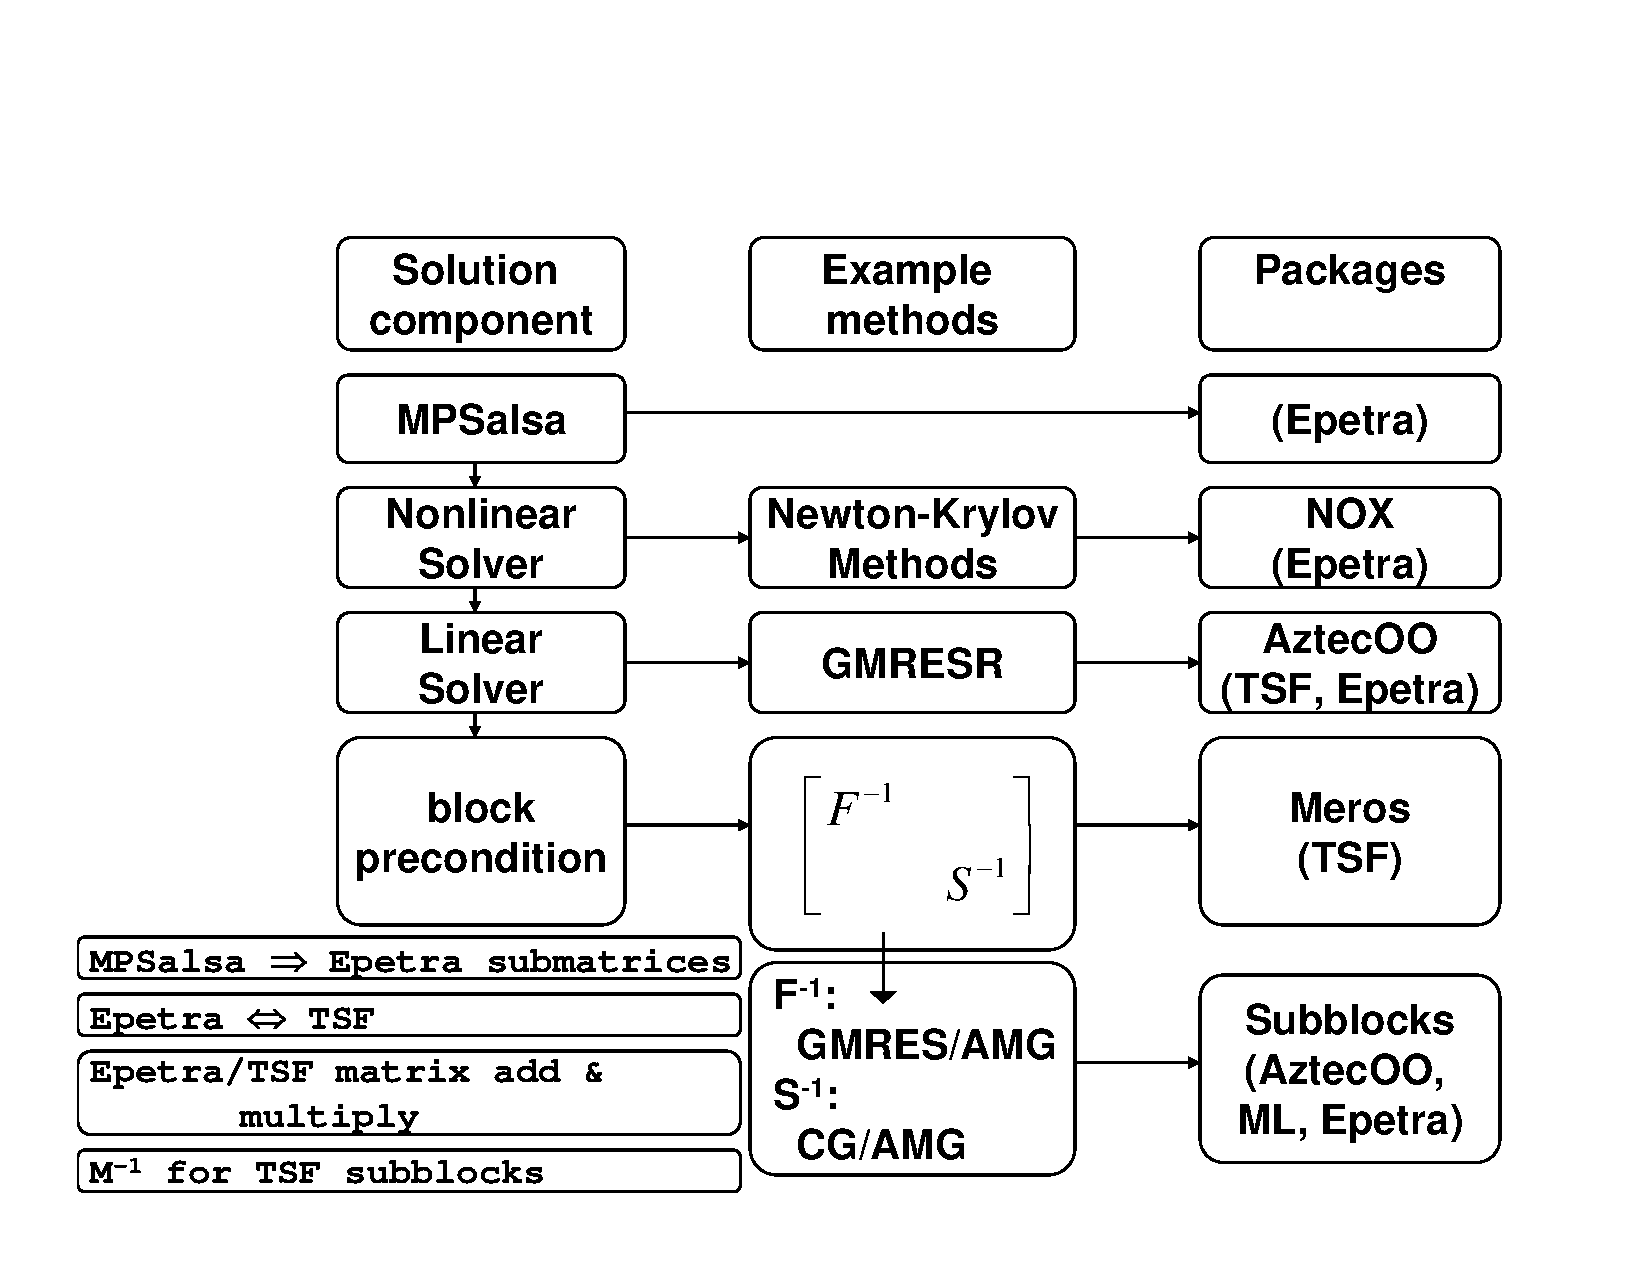
\includegraphics[height=3.5in]{../CommonFiles/MerosBlockDiagram}
\end{center}
\caption{\label{Figure:MerosBlockDiagram}Meros Interaction Diagram}
\end{figure}
illustrates the collaboration and use of Trilinos packages by Meros
in the context of MPSalsa~\cite{MPSalsa-User-Guide}, a reacting flow modeling
application. It is also worth noting that Meros was integrated into
the Trilinos framework using the ``new\_package'' package.  Integration
took less that one day.


\section{Software Engineering Issues}
\label{sect:SQA}
As computer modeling and simulation play an increasingly important
role in engineering and science, a critical issue is software
quality.  Multiple issues are important, but they can be summed up as
follows: {\it If computer modeling and simulation is to be on the critical path 
of engineering and scientific processes, those who rely on our software must
 have confidence in our computational
results.}  It is worth noting that, although much of the work we do to
improve software quality is technical in nature, ultimately it is our
ability to instill trust in our clients that determines whether or not
our software will be used in a production environment.

Much of Trilinos was developed under funding from the Advanced
Scientific Computing Initiative (ASCI).  A major focus of ASCI is
Software Quality Engineering (SQE), which is the set of practices for
ensuring that
high-quality, relevant software is produced, and that software
processes are well-defined, documented and followed.  The present ASCI
SQE practices for Sandia National Laboratories are defined
in~\cite{ASCISQE2003}.  This document describe 47 practices that must
be adopted by each major software project receiving ASCI funding.
These practices cover areas such as software requirements, design,
implementation and maintenance, project management, tracking and
oversight, verification and validation, training and risk management. 

One of the most important goals of Trilinos is to minimize the work
of SQE for the individual package development teams.  Given
that each package is typically written by five or fewer people,
implementation of the ASCI SQE process by each package team would be
almost impossible.  Fortunately, the Trilinos infrastructure
can address the majority of the ASCI SQE practice, fully or
partially.  Table~\ref{table:practices} highlights how Trilinos aids
package developers with some of the 47 practices listed in~\cite{ASCISQE2003}.
Details of Trilinos vs. package responsibilities is presented 
in~\cite{Trilinos-Dev-Guide-II}.   In general, only those practices that are truly
unique to a package are primarily package responsibilities.  This gives
package developers the ability to focus on the core issues of
algorithm design and implementation, and package level documentation
and testing.
\begin{table}
\begin{center}
\begin{tabular}{|p{1.75in}|p{2.75in}|}\hline
\multicolumn{1}{|c|}{Trilinos Service} &
\multicolumn{1}{|c|}{SQE Practices Impact}\\\hline
Yearly Trilinos User Group Meeting (TUG) and Developer Forum: Trilinos Users
and Developers gather once a year for tutorials, package feature updates,
user/developer requirements discussion and developer training. &  
\begin{itemize}
\item All steps of the Requirements including gathering, derivation,
documentation, feasibility, etc. 
\item User training.
\item Developer training.
\end{itemize} \\\hline
Monthly Trilinos leaders meetings: Trilinos leaders, including package
development leaders, key managers, funding sources and other
stakeholders participate in monthly phone meetings to discuss any
timely issues related to the Trilinos Project. &
\begin{itemize}
\item Requirements tracking.
\item Developer Training.
\item Design reviews.
\item Policy decisions across all development phases.
\end{itemize}\\\hline 
Trilinos and package mail lists:  Trilinos lists for leaders,
announcements, developers, users, checkins and similar lists at the package level
support a variety of communication.  All lists are archived, providing
critical artifacts for assessments and audits. &
\begin{itemize}
\item Developer, user and client communication.
\item Repository of requirements, design and testing artifacts.
\item Announcement and documenting of releases.
\end{itemize}\\\hline
Trilinos and Trilinos3PL source repositories:  All source code,
development and user documentation is retained
and tracked. In addition,  reference versions of all external
software, including BLAS, 
LAPACK, Umfpack, etc. are retained in Trilinos3PL.&
\begin{itemize}
\item Source management. 
\item Versioning.
\item Third-party software management.
\end{itemize}\\\hline
Trilinos Bugzilla Database:  Supports collection, tracking and
management of requirements,
enhancements and software faults.&
\begin{itemize}
\item Requirements gathering and tracking.
\item Customer support.
\end{itemize}\\\hline
Trilinos {\tt configure} script and M4 macros: The Trilinos {\tt
configure}  script and related macros support
portable installation of Trilinos and its packages.. &
\begin{itemize}
\item Portability.
\item Software release.
\end{itemize}\\\hline
Trilinos test harness: Trilinos provides a base testing plan and 
automated testing across
multiple platforms, plus creation of testing artifacts. Test harness
results are used to derive a variety of metrics for SQE.&
\begin{itemize}
\item Pre-checkin and regression testing.
\item Software metrics. 
\end{itemize}\\\hline
\end{tabular}
\caption{\label{table:practices} Trilinos Framework support of package
SQE practices}
\end{center}
\end{table}


\section{Conclusions}

In this article we have presented an overview of Trilinos, a 
framework for the development and ongoing support of mathematical
software libraries.  By defining, documenting and prototyping its
package architecture, Trilinos 
provides a ready-made infrastructure that substantially reduces the cost of
mathematical software development.  As a result, Trilinos
has grown rapidly and is able to continue its growth in a scalable
way.  Furthermore, interoperability of packages supports a broad set
of new solvers for coupled multi-physics
applications that are a critical requirement for advanced high-fidelity
simulations.  Finally, the package-oriented delivery of services by
Trilinos for source management, communication, issue tracking,
configuration management and regression testing allow package
developers to readily obtain a high level of SQE support at minimal
cost. 


{\bsinglespace
\bibliographystyle{acmtrans}
\nopagebreak
\scriptsize
\bibliography{../CommonFiles/TrilinosBibliography}
\esinglespace}

\begin{received}
Received: ????; revised: ???; accepted: ???
\end{received}
\end{document}

 
